\documentclass{beamer}
\setbeamertemplate{navigation symbols}{}

\usepackage{beamerthemeshadow}
\setbeamertemplate{caption}[numbered]

\hypersetup{colorlinks}

\def\gw#1{gravitational wave#1 (GW#1)\gdef\gw{GW}}
\def\ns#1{neutron star#1 (NS#1)\gdef\ns{NS}}

\newcommand{\red}[1]{{\color{red}{#1}}}

\begin{document}
\title{BHextractor / PCA Update \& Notes}
%\subtitle{Burst Call Oct 8$^{\text{th}}$ 2014}  
\author{James A. Clark}
%\institute{Georgia Institute Of Technology}
\date{} 

\begin{frame}[plain]
\titlepage
\end{frame}

%\begin{frame}\frametitle{Table of contents}\tableofcontents
%\end{frame} 

\section{Projects}

\begin{frame}

    \frametitle{Things we have going on / I know about}
    \begin{itemize}
        \item Continuing BHextractor / Sant-Cugant work
            \begin{itemize} 
                \item `September paper'
            \end{itemize}
        \item NR catalogue studies
            \begin{itemize} 
                \item PCAT-style clustering
                \item Waveform / parameter Interpolation
            \end{itemize}
        \item Analytic Catalogue Studies
            \begin{itemize}
                \item PCA Characterization \& Exploration 
            \end{itemize}
    \end{itemize}

\end{frame}

\section{BHextractor}

\begin{frame}
    \frametitle{BHextractor: previous work}
    \begin{itemize}
        \item Small (~20 waveforms) catalogues (Q, HR, RO3)
        \item Used all available harmonics, constructed optimally oriented
            (face-on) waveforms
        \item PCs computed from truncated, aligned \& SNR-scaled waveforms
        \item Evidence computed in old SMEE matlab script for each catalogue
        \item No sky-location search, no time-search, no mass-search
        \item Single IFO
        \item Reasonable success in distinguishing the more `distinct' waveforms
        \item No attempt at parameter estimation; goal was \emph{only}
            separation of catalogues
    \end{itemize}
\end{frame}

\begin{frame}
    \frametitle{BHextractor: Recent / On-going}
    \begin{itemize}
        \item N. Mangini (now left): started looking at PCs with complex ($h_+ -
            i h_{\times}$) waveforms and handling inclination
        \item D. Leininger (Glasgow summer): investigated sky-localisation and
            multi-IFO application
        \item A. Lombardi (UMass):  understand / incorporate search over total
            mass (amplitude scaling \& $\sim$resampling)
        \item S. Kimbrell: tentative plan is to repeat \& extend Sant-Cugant
            study using {\tt LALInference} implementation of SMEE.  J. Powell
            working to publish a branch of {\tt LAL} with the SMEE edits.
    \end{itemize}

    Note: we also need
    \begin{enumerate}
        \item {\bf careful treatment of orientation \& harmonics}
        \item a consistent and meaningful way to define catalogues (do we even
            \emph{want} catalogues?)
        %\item Some statement on physical parameters
    \end{enumerate}

\end{frame}

\section{Waveform Clustering}

\begin{frame}
    \frametitle{Waveform Clustering}
    `PCAT': algorithm for glitch classification in detchar:
    \begin{enumerate}
        \item Construct a \emph{single} catalogue of all waveforms
        \item Perform PCA
        \item Use GMM to identify clusters of principle component
            `scores'
        \item Clusters in PC-score space represent morphologically
            similar waveforms
    \end{enumerate}
    So far: prototype script to generate a catalogue
        comprised of sine-Gaussians \& chirps (randomised params),
        perform PCA / clustering and identify the different families
    \begin{itemize}
        \item \emph{Potential} use in constructing morphologically similar
            catalogues
        \item \emph{Potential} use in grouping together similar waveforms for
            constructing sensible interpolants in PCA-based waveform
            interpolation \dots
    \end{itemize}
\end{frame}

\begin{frame}
    \frametitle{Waveform Clustering Demo / Prototype}

    \begin{columns}[]
        \column{0.5\textwidth}
        \begin{center}
        \begin{figure}
            \vspace*{-0.5cm}
            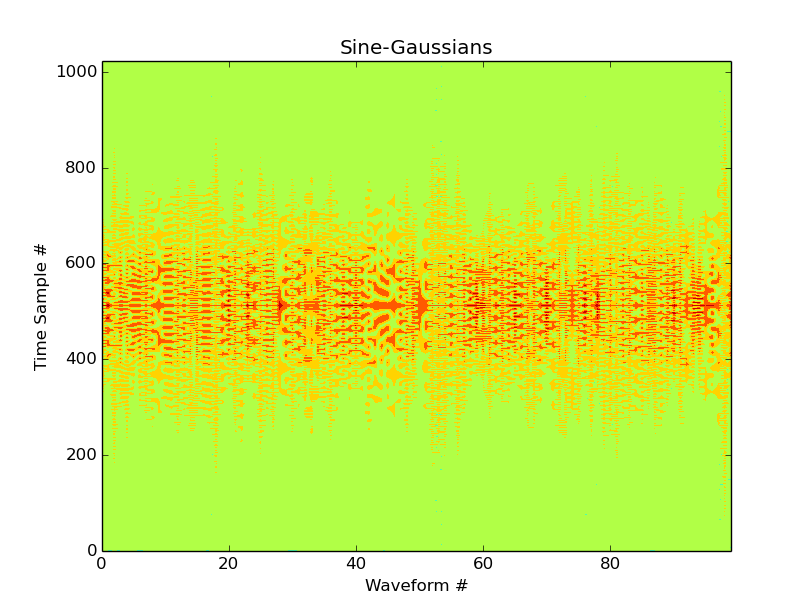
\includegraphics[scale=0.3]{sinegaussians.png} 
            %\caption{Sine-Gaussians}
        \end{figure}
        \end{center}

        \column{0.5\textwidth}
        \begin{center}
        \begin{figure}
            \vspace*{-0.5cm}
            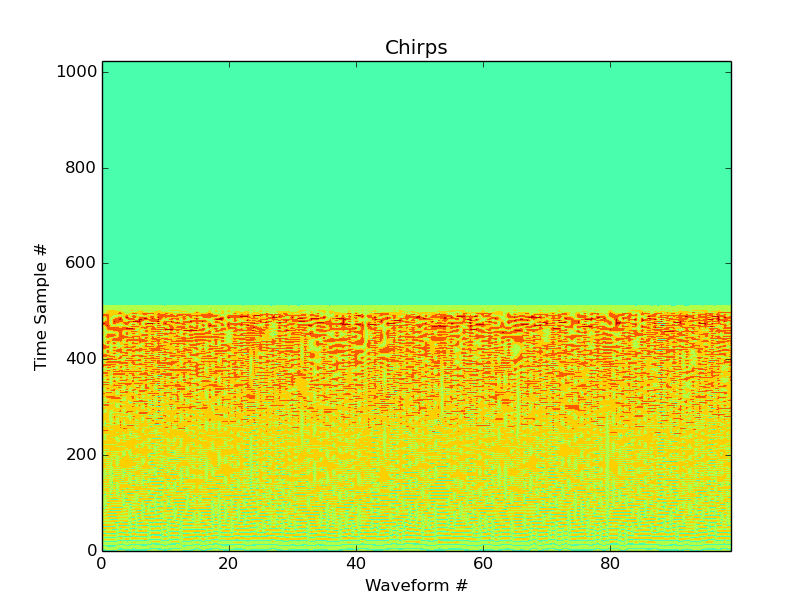
\includegraphics[scale=0.3]{chirps.png} 
            %\caption{Chirps}
        \end{figure}
        \end{center}
    \end{columns}

500 waveforms of each type: algorithm identifies 2 distinct waveform
morphologies from clustering the PCA scores with 48/52\% membership, using just
the first 50 PCs.

\end{frame}

\section{Waveform Interpolation}

\begin{frame}
    \frametitle{PCA \& Parameter Estimation / Waveform Interpolation}
    Finally understand the fundamental idea behind waveform interpolation and
    connection with parameter estimation!
    \begin{enumerate}
        \item Build catalogue of waveforms with varying (say) $q=m_1/m_2$;
            catalogue: $\{h(t|q_1),~h(t|q_2),~\dots\}$
        \item Compute PCs $U_i$ and coefficients $\beta_i$ where waveform is
            \begin{equation}
                h(t|q) = \sum_{i=1} \beta_i U_i
            \end{equation}
        \item Realise we can interpolate \emph{each} $\beta_i$ as a function of
            $q$
        \item E.g., have discretely sampled $\{\beta_1(q)\} = \{\beta_1(q_1),~
            \beta_1(q_2),~\dots\}$ (and similarly for $\beta_2,~\dots$)
        \item So we can get $h(t|q')$ for arbitrary $q'$ by interpolating
            $\beta(q)$
    \end{enumerate}

\end{frame}

\begin{frame}
    \frametitle{PCA \& Parameter Estimation / Waveform Interpolation}
    Example: Q-series has mass ratios $q=\{1.  ,  1.15,  1.3 ,  1.45,  1.5 ,  1.6
    ,  1.75,  1.9 ,  2.  , 2.05,  2.2 ,  2.35,  2.5\}$; interpolate to find
    $h(t|q=2.1)$:

    \begin{columns}[]
        \column{0.5\textwidth}
        \begin{center}
        \begin{figure}
            \vspace*{-0.5cm}
            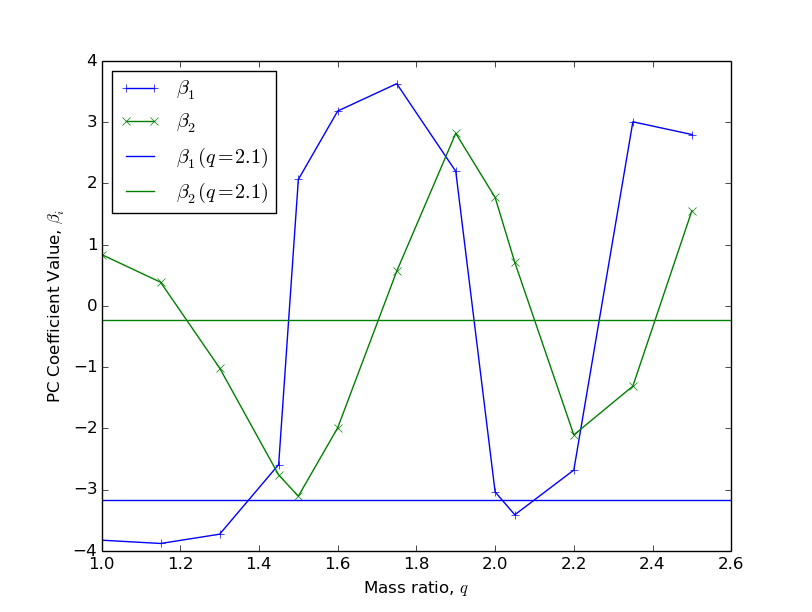
\includegraphics[scale=0.3]{PC_coeff_example.png} 
        \end{figure}
        \end{center}

        \column{0.5\textwidth}
        \begin{center}
        \begin{figure}
            \vspace*{-0.5cm}
            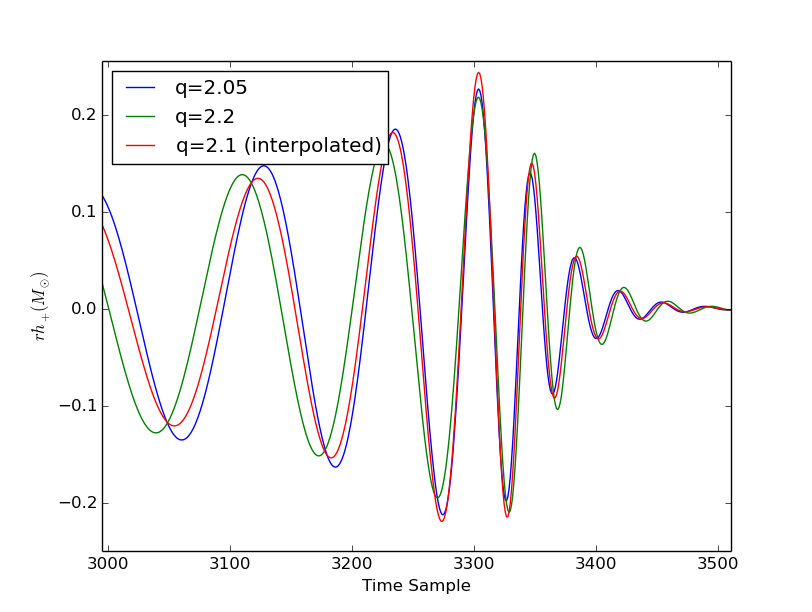
\includegraphics[scale=0.3]{waveform_interp_example.png} 
        \end{figure}
        \end{center}
    \end{columns}

\end{frame}

\begin{frame}
    \frametitle{PCA \& Parameter Estimation / Waveform Interpolation}
    \small
    \begin{itemize}
        \item 1-D interpolation between (e.g.) mass ratios $\sim$trivial
        \item To be useful, we need multivariate interpolation to handle spins
            and internal orientation angles
        \item \url{http://en.wikipedia.org/wiki/Multivariate_interpolation}
        \item See also \S8 of arXiv:1402.4146 - seems to be supported in
            Mathematica, Matlab but still casting around for pythong solutions
        \item Any local experience / expertise with \emph{tensor product spline
            interpolation}???
        \item Note: it may well be useful / necessary to group like-waveforms
            together, essentially into distinct catalogues, each with their own
            interpolants; this is the \emph{potential}\footnote{no idea if this
            will be sensitive to different BBH waveforms!} use of the PCAT-style
            clustering
    \end{itemize}

\end{frame}

\begin{frame}
    \frametitle{PCA \& Parameter Estimation / Waveform Interpolation}
    \small
    Other thoughts / concerns:
    \begin{itemize}
        \item Do we want to be stuck in the time-domain? (The SEOBNR ROMs are
            F-domain).  F-domain is \emph{strongly} preferred for any kind of
            parameter estimation.
        \item How can we use PCA \& interpolation to identify under-sampled
            regions of parameter space in NR simulations?
        \item \emph{What do we do with higher modes \& unknown source
        orientation?}
        \begin{itemize}
            \item Include orientation in PCA?  Seems unfeasible / unnecessary /
                ugly
            \item PCA \& interpolants for \emph{each} mode?
        \end{itemize}
    \end{itemize}

\end{frame}

\begin{frame}
    \frametitle{Where Next / Plans}
    \small
    \begin{itemize}
        \item Sant-Cugant study using LALInference implementation of SMEE
            \begin{itemize}
                \item will get evidence for `catalogues' and posterior samples
                    for $\beta_i$; can we say something useful using these
                    without going as far as waveform interpolation?
            \end{itemize}
        \item `September paper':  overhaul of Sant-Cugant study 
        \item Clustering: tidy up demo script, understand and charaterise
            clustering behaviour, apply to BBH waveforms
        \item Interpolation: understand implementation of tensor spline interpolation
            \begin{itemize}
                \item Call to be scheduled with J. Veitch next week to talk
                    about what we could do
                \item Particularly interested in identifying under-sampled
                    regions of parameter space to guide NR simulations
                \item B. Day's studies with EOBNR \& PCA could be a good
                    test-bed for interpolation studies
            \end{itemize}
    \end{itemize}
\end{frame}

\begin{frame}
    \frametitle{Wavelets?}
    Maybe something useful to do with wavelet scaleograms (a la `eigenfaces')?

    Left side: Q-series, face-on; Right side: RO3-series, edge-on
    \begin{figure}
        \center
        \scalebox{0.15}{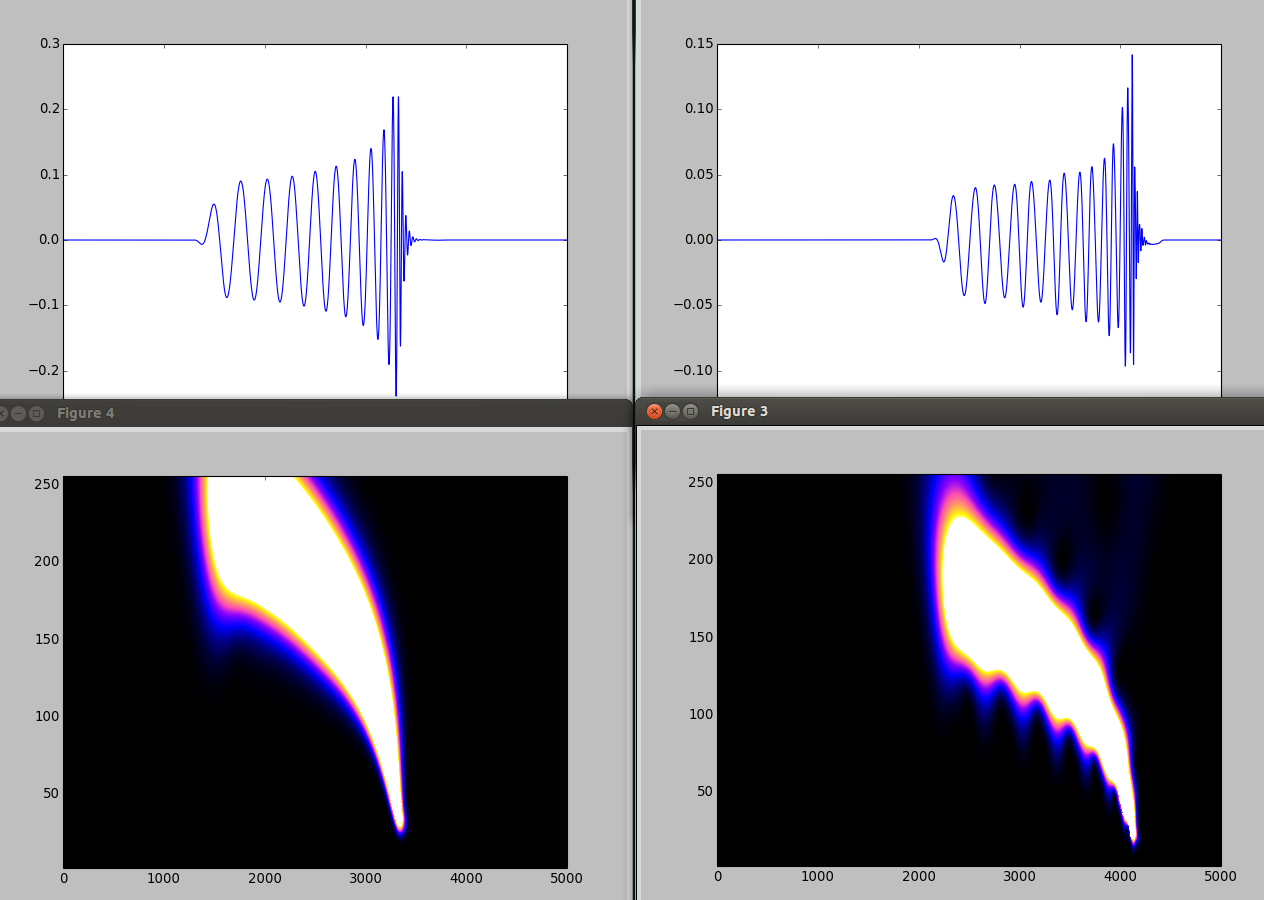
\includegraphics{wavelets.png}}
    \end{figure}

\end{frame}

\end{document}
